% !TEX root = ../main.tex
% ══════════════════════════════════════════════════════════════
\chapter{Contexte, problématique et cadrage du projet}
% ══════════════════════════════════════════════════════════════
\begingroup
\let\clearpage\relax
\startcontents[chapters]
\printcontents[chapters]{}{1}{\section*{Plan}}
\endgroup
\newpage

\section*{Introduction}
\justifying
\phantomsection
\addcontentsline{toc}{section}{Introduction}

Ce chapitre présente l'organisme d'accueil et analyse le système d'information utilisé pour la gestion des mobilités internationales. Il en dégage la problématique et la solution envisagée, précise les besoins du système, puis présente le cadrage retenu pour conduire le projet.

% ─────────────────────────────────────────────────────────────
\section{Présentation de l'organisme d'accueil}
% ─────────────────────────────────────────────────────────────

Ce stage a été effectué au sein de Toulouse INP-ENSEEIHT, école d'ingénieurs publique toulousaine, et plus précisément dans son service des Relations Internationales. Cette section présente d'abord l'établissement d'accueil, puis le service dans lequel le stage a été réalisé.

\subsection{Présentation de Toulouse INP-ENSEEIHT}

Toulouse INP-ENSEEIHT est une école publique d'ingénieurs, située à Toulouse et rattachée à l'Institut national polytechnique de Toulouse. Elle forme chaque année des ingénieurs, des étudiants en master et en doctorat dans trois spécialités : Sciences du Numérique (SN), Électronique–Énergie électrique–Automatique (EEEA) et Mécanique des Fluides, Énergétique \& Environnement (MFEE).

L'école collabore avec plusieurs laboratoires de recherche, notamment IMFT, IRIT, LAAS et LAPLACE, et entretient des liens avec de nombreux partenaires industriels. Le développement à l'international fait partie de ses priorités : elle agrandit régulièrement son réseau d'universités partenaires et favorise les séjours à l'étranger pour ses étudiants~\cite{enseeiht_presentation}.

\subsection{Le service des relations internationales}

Le service des Relations Internationales (RI) gère les échanges entre l'ENSEEIHT et ses partenaires à l'étranger. Son rôle est à la fois stratégique et opérationnel : il s'occupe des accords de partenariat, mais aussi du suivi quotidien des mobilités étudiantes. Ses activités se répartissent en six domaines~\cite{enseeiht_international}.

\textbf{La gestion des partenariats académiques} : gestion d'un réseau d'accords bilatéraux avec des universités étrangères, incluant les programmes d'échange et les doubles diplômes, avec suivi des places disponibles par accord et par département.

\textbf{L'organisation des mobilités sortantes} : organisation de la campagne annuelle de sélection des étudiants de l'ENSEEIHT partant à l'étranger, depuis la publication des destinations jusqu'à la validation des affectations~\cite{enseeiht_sortante}.

\textbf{L'accueil des mobilités entrantes} : inscription et suivi des étudiants étrangers accueillis à l'ENSEEIHT dans le cadre des accords de partenariat~\cite{enseeiht_entrante}.

\textbf{L'accompagnement administratif et pédagogique} : aide aux étudiants pour les procédures de départ, suivi des aspects financiers et vérification de la conformité des dossiers.

\textbf{Le reporting CTI} : suivi des mobilités entrantes et sortantes pour les audits de la Commission des Titres d'Ingénieur, qui exige une durée minimale de séjour à l'étranger pour l'obtention du diplôme.

\textbf{La gestion des programmes courts} : suivi des étudiants participant à des summer schools, séjours linguistiques ou autres programmes de courte durée, qui peuvent être comptabilisés dans la durée de mobilité sous certaines conditions~\cite{enseeiht_programmes_courts}.

Ces activités nécessitent de traiter chaque jour des données venant de plusieurs sources différentes, dans des formats qui ne sont pas toujours compatibles. C'est ce problème qui est au cœur du projet présenté dans ce rapport.

% ─────────────────────────────────────────────────────────────
\section{Analyse du système d'information interne}
% ─────────────────────────────────────────────────────────────

Avant de proposer une solution, il faut d'abord comprendre comment le service RI fonctionne et quels outils il utilise. Cette section décrit les systèmes en place, puis présente les problèmes que leur utilisation crée au quotidien.

\subsection{Les outils en place}

Le service RI utilise quatre outils distincts, qui ne communiquent pas entre eux.

\subsubsection{QS MoveON}

MoveON est l'outil principal du service RI. Il permet de gérer les accords bilatéraux, les quotas INP et les candidatures des étudiants. Il dispose d'une API REST qui permet d'extraire les données~\cite{qs_moveon}. Mais il ne prend pas en compte les résultats académiques des étudiants, ne propose pas d'aide pour la sélection, et ne couvre ni les stages ni les autres éléments du parcours individuel.

\subsubsection{Pégase}

Pégase est le système d'information académique de Toulouse INP. Il regroupe les données des étudiants : inscription, département, niveau, parcours pédagogique et notes — en particulier le GPA trimestriel, qui sert à classer les candidatures. Ces informations sont essentielles pour la gestion des mobilités. Les données sont accessibles via une API, mais il n'existe aucun lien direct avec MoveON.

\subsubsection{Eudonet}

Eudonet est l'outil utilisé pour gérer les conventions de stage. Il contient les informations sur les stages nationaux et internationaux : entreprise d'accueil, dates et durée~\cite{eudonet_crm}. Ces données entrent dans le calcul de la durée de mobilité, mais elles ne sont pas reliées aux autres systèmes.

\subsubsection{Les fichiers Excel}

Pour pallier les manques des trois outils précédents, le service RI utilise des fichiers Excel qu'il gère lui-même : suivi des quotas par département, gestion des mobilités entrantes, calcul des durées et suivi des programmes courts. Même avec une personne rigoureuse, cette méthode reste risquée : erreurs de saisie, oublis de mise à jour, fautes de frappe, incohérences entre fichiers — ces problèmes sont difficiles à repérer et peuvent avoir des conséquences directes sur le déroulement de la campagne.

\subsection{Limites structurelles}

La figure~\ref{fig:systeme_existant} montre l'organisation actuelle du service RI : quatre outils utilisés séparément, sans aucune connexion automatique entre eux. Chaque transfert de données se fait manuellement.

\begin{figure}[H]
\centering
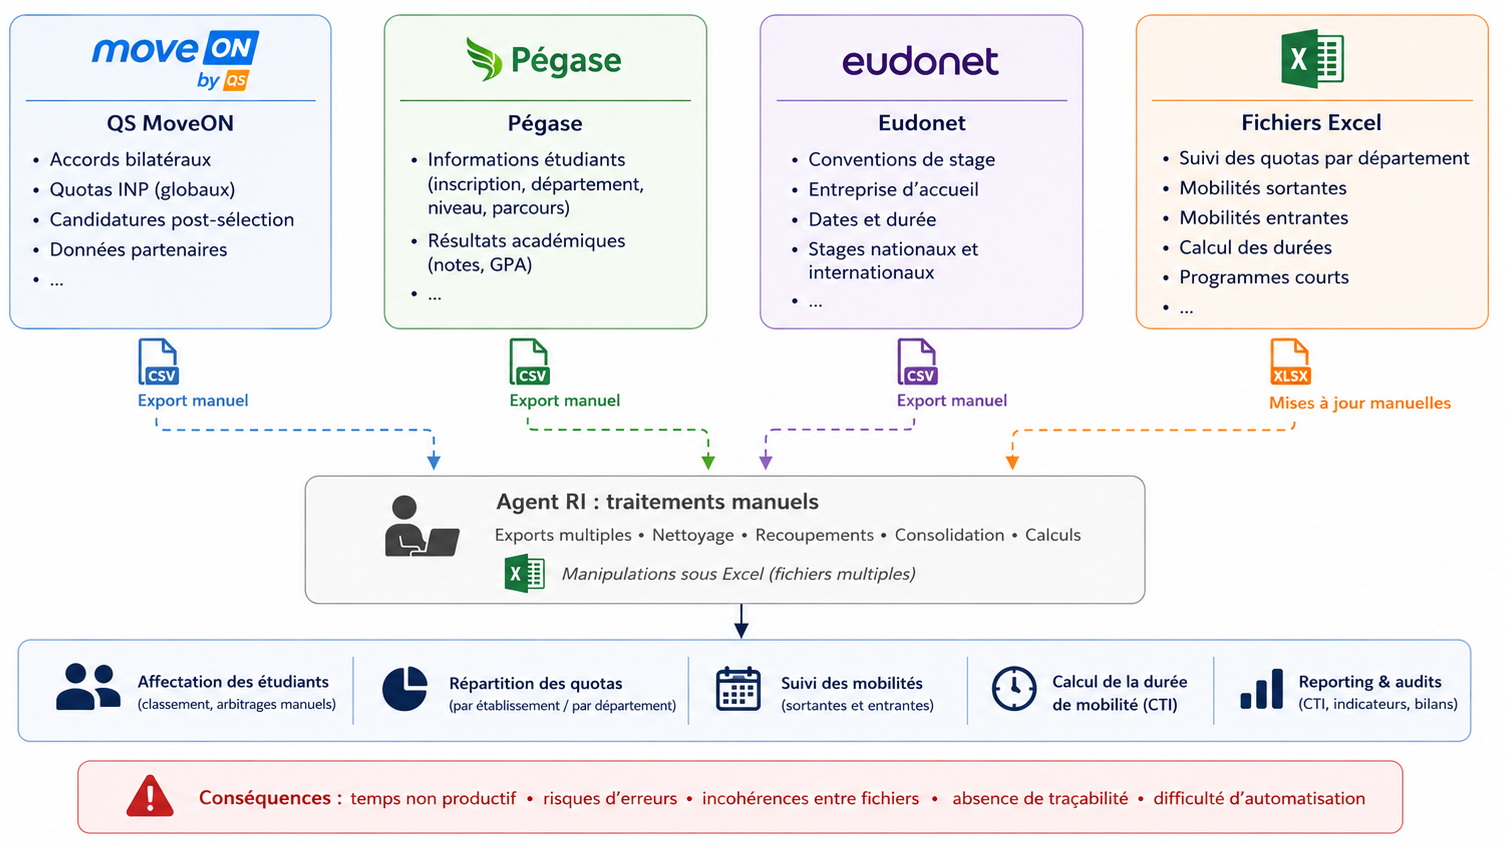
\includegraphics[width=0.90\textwidth]{figures/systemes/systeme-existant.png}
\caption{Système d'information existant du service RI}
\label{fig:systeme_existant}
\end{figure}

Cette absence de communication entre les outils crée plusieurs problèmes qui reviennent à chaque campagne.

\begin{itemize}
    \item \textbf{Des exports manuels à chaque étape.} Comme les outils ne communiquent pas entre eux, chaque consolidation de données nécessite des exports depuis plusieurs plateformes, puis une mise en forme dans Excel. Ce travail est long et source d'erreurs.

    \item \textbf{Une sélection sans règles fixes.} Les candidats sont classés manuellement à partir d'un tableau de GPA. En cas d'égalité ou de cas particulier, c'est l'agent RI qui tranche, et sa décision peut changer d'une année à l'autre sans qu'il y ait de trace écrite.

    \item \textbf{Des quotas insuffisamment détaillés.} MoveON ne gère les places qu'à l'échelle de l'INP global, sans distinguer les établissements qui le composent. La répartition par établissement (dont l'ENSEEIHT), puis par département pédagogique, est faite manuellement dans Excel, sans vérification de cohérence.

    \item \textbf{Des mobilités complémentaires non suivies.} Les summer schools, séjours linguistiques et programmes courts n'ont pas de place dans les outils existants. Pour les inclure dans le calcul de la durée de mobilité, l'agent doit s'en souvenir lui-même — ce qui n'est pas fiable.

    \item \textbf{Un calcul de durée de mobilité entièrement manuel et coûteux en temps.} Pour calculer la durée de mobilité d'un étudiant, il faut rassembler des données réparties dans trois systèmes différents (MoveON, Pégase, Eudonet) et les recouper à la main dans Excel. Selon les échanges avec le service RI, cette consolidation représente de l'ordre d'une dizaine de minutes par dossier, soit plusieurs journées de traitement cumulées à l'échelle d'une promotion de 300 étudiants — sans compter le risque d'oubli d'une période de mobilité à chaque manipulation. Cette opération ne peut pas être automatisée tant qu'il n'existe pas de source de données unifiée.
\end{itemize}

% ─────────────────────────────────────────────────────────────
\section{Problématique et solution envisagée}
% ─────────────────────────────────────────────────────────────

Cette section formule la problématique centrale du projet à partir du constat précédent, puis présente la solution envisagée dans ses grandes lignes. 

\subsection{Problématique}

Le service RI utilise plusieurs outils qui ne communiquent pas entre eux. Chaque transfert de données se fait à la main, l'affectation des étudiants n'a pas de règle fixe, et il n'existe pas de moyen simple de calculer la durée de mobilité. Cinq problèmes restent sans solution :

\begin{itemize}
  \item Les données sont dispersées entre plusieurs systèmes et ne peuvent pas être consultées depuis un seul endroit.
  \item Les quotas ne descendent pas jusqu'au niveau département, alors que c'est ce niveau qui détermine qui peut partir et où.
  \item La sélection des candidats se fait à la main, sans règle définie à l'avance.
  \item Le calcul de la durée de mobilité oblige à rassembler des données venant de plusieurs sources différentes.
  \item Les étudiants n'ont pas d'aide pour choisir leurs destinations.
\end{itemize}

C'est à partir de ce constat que se formule la question centrale du projet :

\begin{quote}
\textit{Comment concevoir une plateforme intégrée qui automatise le processus de gestion des mobilités internationales à l'ENSEEIHT, depuis la centralisation des données multi-sources jusqu'à l'affectation algorithmique, tout en garantissant la conformité CTI et l'aide à la décision des étudiants ?}
\end{quote}

\subsection{Solution envisagée}

La réponse envisagée est le développement d'une plateforme propre au service RI. Elle ne remplace pas les outils existants, mais se connecte à eux pour récupérer les données automatiquement. Elle doit permettre de gérer les quotas par département, de classer et affecter les étudiants selon des règles définies à l'avance, de calculer la durée de mobilité de façon automatique, et d'aider les étudiants à choisir leurs destinations. L'objectif est de centraliser les données et de réduire le travail manuel.

% ─────────────────────────────────────────────────────────────
\section{Besoins du système}
\label{sec:besoins-systeme}
% ─────────────────────────────────────────────────────────────

Cette section décrit les principales fonctionnalités attendues du système, les exigences non fonctionnelles associées, ainsi que les profils utilisateurs et le périmètre de réalisation retenu pour ce projet.

\subsection{Besoins fonctionnels}

Les besoins fonctionnels décrivent les principales fonctionnalités attendues du système afin de répondre aux problématiques identifiées au sein du service RI. Ils couvrent à la fois les fonctionnalités opérationnelles et les fonctionnalités intelligentes.

\subsubsection{Fonctionnalités opérationnelles}

Le système prend en charge les opérations suivantes, qui couvrent l'ensemble du cycle de gestion des mobilités internationales, de l'import des données jusqu'à l'archivage des résultats.

\begin{itemize}
    \item \textbf{BF01 --- Intégration des données} : import depuis MoveON, Pégase et Eudonet via API REST, et depuis des fichiers Excel pour les sources sans API. Chaque import inclut une détection de doublons, une validation des formats et un mécanisme de fallback Excel en cas d'indisponibilité d'une API.
    \item \textbf{BF02 --- Gestion des accords et quotas} : import des accords depuis MoveON et gestion de la répartition locale des places par département N7, avec possibilité d'ajustement manuel par le service RI.
    \item \textbf{BF03 --- Algorithme d'affectation} : pré-affectation automatique basée sur le GPA, les vœux ordonnés et les quotas par département, avec interface de supervision et d'ajustement.
    \item \textbf{BF04 --- Suivi de la durée de mobilité} : calcul automatique de la durée totale de mobilité de chaque étudiant, par agrégation des séjours académiques, stages et expériences complémentaires validées.
    \item \textbf{BF05 --- Mobilités complémentaires} : les étudiants déclarent leurs expériences et déposent les justificatifs nécessaires, puis le service RI se charge de la validation des dossiers.
    \item \textbf{BF06 --- Mobilités entrantes} : import via template Excel et suivi administratif granulaire.
    \item \textbf{BF07 --- Historisation} : les données d'une campagne clôturée passent en lecture seule. Aucune exécution ultérieure ne peut modifier les résultats d'une année passée.
    \item \textbf{BF08 --- Reporting et enquêtes CTI} : calcul automatique des indicateurs requis pour les enquêtes annuelles de la Commission des Titres d'Ingénieur — nombre et pourcentage d'étudiants mobiles, durée moyenne de mobilité, répartition des destinations — ainsi qu'export des rapports de conformité correspondants.
\end{itemize}

\subsubsection{Fonctionnalités intelligentes}

En complément des fonctionnalités opérationnelles, le système intègre deux modules intelligents qui améliorent l'expérience étudiant sans solliciter le service RI.

\begin{itemize}
    \item \textbf{BF09 --- Moteur de recommandation} : suggestions de destinations basées sur le GPA, le département et l'historique des affectations, pour orienter les choix de l'étudiant avant la saisie dans MoveON.
    \item \textbf{BF10 --- Assistant virtuel (chatbot RAG)} : agent conversationnel répondant aux questions procédurales à partir de la documentation institutionnelle, sans solliciter le service RI.
\end{itemize}

\subsection{Besoins non fonctionnels}

Au-delà des fonctionnalités métier, le système doit également répondre à plusieurs exigences techniques et organisationnelles. Ces besoins non fonctionnels concernent notamment la sécurité, la performance, l'intégrité des données et l'intégration avec l'environnement existant.

\begin{itemize}
    \item \textbf{BNF01 --- Interopérabilité} : le système doit s'intégrer sans rupture dans l'écosystème existant via des adaptateurs REST dédiés à chaque source. En cas d'indisponibilité d'une API, un fallback par import Excel garantit la continuité opérationnelle.

    \item \textbf{BNF02 --- Intégrité des données} : les données provenant de sources hétérogènes peuvent être incohérentes ou dupliquées. Une validation stricte est appliquée à chaque import — contrôle de format, détection de doublons, cohérence inter-sources. Toute donnée rejetée est tracée dans un rapport d'import avec la raison précise, pour correction ciblée.

    \item \textbf{BNF03 --- Sécurité et RGPD} : authentification via le SSO institutionnel, gestion stricte des rôles (étudiant vs administrateur), chiffrement des données sensibles. Un étudiant n'accède qu'à son propre dossier.

    \item \textbf{BNF04 --- Performance} : le temps de réponse de l'API pour les endpoints courants doit être inférieur à 200~ms sous une charge de 50 utilisateurs simultanés. L'algorithme d'affectation doit s'exécuter en moins de 30 secondes pour une promotion de 300 étudiants. Les traitements lourds — algorithme d'affectation, calculs CTI — sont exécutés de façon asynchrone en arrière-plan pour ne pas bloquer l'interface.

    \item \textbf{BNF05 --- Disponibilité} : s'agissant d'un système institutionnel sollicité lors de périodes de campagne critiques (ouverture des vœux, publication des résultats), une disponibilité cible de 99~\% hors fenêtres de maintenance planifiées est visée, appuyée par une politique de sauvegarde permettant une reprise rapide en cas d'incident.

    \item \textbf{BNF06 --- Scalabilité} : séparation entre données actives et données archivées en lecture seule pour absorber la croissance annuelle du volume historique et les pics de connexion lors des moments clés de campagne.

    \item \textbf{BNF07 --- Ergonomie} : l'interface adapte sa navigation et ses fonctionnalités au rôle de l'utilisateur connecté, réduisant les erreurs de manipulation.

    \item \textbf{BNF08 --- Traçabilité} : toute action importante — import, modification d'affectation, validation, transition de phase — est enregistrée avec l'identité de l'auteur et l'horodatage dans un journal d'audit persistant en écriture seule.
\end{itemize}

\subsection{Profils utilisateurs et périmètre de réalisation}

Cette sous-section présente les profils d'utilisateurs du système, puis définit le périmètre de réalisation retenu pour ce projet.

\subsubsection{Profils utilisateurs}

Deux profils utilisent le système, avec des besoins très différents.

\textbf{L'administrateur} — c'est-à-dire le service RI — pilote la campagne de bout en bout. Il supervise les imports, configure les quotas, ajuste les propositions d'affectation, instruit les demandes de mobilités complémentaires et produit les rapports CTI. Le système prend en charge les tâches répétitives, mais toute décision finale reste sous sa responsabilité, et chaque intervention manuelle est tracée.

\textbf{L'étudiant} consulte les destinations disponibles, reçoit des recommandations personnalisées avant de saisir ses vœux dans MoveON, suit l'état de sa candidature, déclare ses expériences complémentaires et vérifie à tout moment si sa durée totale de mobilité atteint le seuil requis pour l'obtention du diplôme. L'assistant virtuel répond à ses questions procédurales sans solliciter le service RI.

\subsubsection{Périmètre de réalisation}

Le développement est organisé en deux niveaux de priorité.

\textbf{MVP — fonctionnalités prioritaires (BF01 à BF08, BNF01 à BNF08)} :
\begin{itemize}
  \item Intégration des données multi-sources (MoveON, Pégase, Eudonet, Excel)
  \item Gestion des accords et quotas par département
  \item Algorithme d'affectation avec validation humaine
  \item Calcul automatique de la durée de mobilité
  \item Gestion des mobilités complémentaires et entrantes
  \item Reporting et enquêtes CTI : indicateurs chiffrés, tableaux de bord analytiques et exports de conformité
  \item Espace étudiant : catalogue, suivi de candidature, déclarations
  \item Sécurité : SSO, contrôle d'accès, audit log
\end{itemize}

\textbf{V2 — fonctionnalités secondaires (BF09, BF10)} :
\begin{itemize}
  \item Moteur de recommandation de destinations personnalisé
  \item Assistant virtuel (chatbot RAG)
\end{itemize}

% ─────────────────────────────────────────────────────────────
\section{Organisation et cadrage du projet}
% ─────────────────────────────────────────────────────────────

Cette section regroupe les éléments qui cadrent la conduite du projet : la méthodologie de gestion de projet retenue, la planification générale et l'environnement de travail utilisé.

\subsection{Méthodologie de gestion de projet}

Le projet s'étend sur six mois dans un contexte où certaines règles métier
n'étaient pas complètement formalisées dès le départ. Trois approches ont été
évaluées avant de retenir la méthodologie la mieux adaptée.

\subsubsection{Méthode en cascade}

La méthode en cascade organise le projet en phases séquentielles et strictement
ordonnées : analyse, conception, développement, test, déploiement. Chaque phase
doit être complètement terminée avant de passer à la suivante.

\textbf{Avantages :} Elle offre une planification claire et une documentation
exhaustive dès le départ, ce qui facilite le suivi et la traçabilité des décisions.

\textbf{Limites dans notre contexte :} Elle impose de geler un cahier des charges
complet avant tout développement. Or, certaines règles métier — notamment la
hiérarchie des quotas et les critères de priorité dans l'affectation — n'étaient
pas entièrement définies au démarrage du projet, rendant cette approche inadaptée.

\subsubsection{Kanban}

Kanban est une méthode de gestion de flux continu, sans itérations fixes. Le
travail est visualisé sur un tableau et les tâches avancent au fur et à mesure
de la disponibilité de l'équipe.

\textbf{Avantages :} Sa flexibilité permet de s'adapter rapidement aux changements
et de traiter les tâches par ordre de priorité sans contrainte de cycle.

\textbf{Limites dans notre contexte :} L'absence d'itérations fixes et de
jalons structurés le rend peu adapté à un projet avec un périmètre défini et
une date de livraison fixe, où une planification rigoureuse est nécessaire.

\subsubsection{Scrum}

Scrum est un cadre agile qui organise le développement en sprints de durée fixe,
avec des événements régulières (planning, review, retrospective) et un backlog
priorisé.

\textbf{Avantages :} Il offre un bon équilibre entre structure et flexibilité :
les priorités peuvent être révisées à chaque sprint, les livraisons sont
incrémentales et validables régulièrement par le service RI.

\textbf{Limites dans notre contexte :} Scrum est conçu pour des équipes. Certains
événements, comme le Daily Scrum ou la rétrospective d'équipe, supposent une
coordination quotidienne entre plusieurs personnes et ne s'appliquent pas tels
quels à un projet porté par une seule développeuse ; ils doivent être adaptés
ou remplacés par des pratiques équivalentes.

\subsubsection{Comparaison et choix retenu}

Le tableau~\ref{tab:methodo_comparaison} compare les trois approches sur des critères objectifs.

\renewcommand{\arraystretch}{1.4}
\begin{table}[H]
\centering
\footnotesize
\begin{tabular}{|p{3cm}|p{3cm}|p{3cm}|p{3cm}|}
\hline
\rowcolor{gray!20}
\textbf{Critère} & \textbf{Cascade} & \textbf{Kanban} & \textbf{Scrum} \\
\hline
Planification & Rigide dès le début & Continue, sans itérations fixes & Sprints fixes avec rétroplanification \\
\hline
Adaptation aux changements & Difficile & Bonne, mais sans rythme structuré & Bonne, intégrée à chaque sprint \\
\hline
Visibilité client & Faible en cours de projet & Modérée & Élevée (Sprint Review) \\
\hline
\end{tabular}
\caption{Comparaison des approches de gestion de projet}
\label{tab:methodo_comparaison}
\end{table}

Au regard de ces trois critères, Scrum est le seul à combiner une planification structurée et une capacité d'adaptation intégrée à chaque itération, tout en offrant la meilleure visibilité pour le service RI. C'est pourquoi \textbf{Scrum} est retenu, pour son équilibre entre structure (sprints de durée
fixe, backlog priorisé) et flexibilité (révision des priorités à chaque sprint,
livraisons incrémentales validables par le service RI). Ce cadre étant conçu
pour une équipe, son application est toutefois adaptée au contexte d'un
développement individuel : certains rôles et événements sont ajustés ou
remplacés par des pratiques équivalentes, comme précisé ci-dessous.

Scrum s'appuie sur des rôles, des artefacts et des événements, présentés
ci-dessous et adaptés au contexte d'un stage individuel.

\subsubsection{Les rôles Scrum}

\begin{itemize}[label=•]
    \item \textit{\textbf{Le Product Owner}} : responsable de la priorisation du backlog et de la validation des livraisons.
    \item \textit{\textbf{Le Scrum Master}} : chargé du suivi de l'avancement, de la levée des blocages et de l'orientation technique.
    \item \textit{\textbf{L'équipe de développement (Development Team)}} : réalise les incréments du produit. Ce rôle est habituellement porté par plusieurs personnes ; dans ce projet, il est assuré par une seule personne, responsable de l'intégralité du développement.
\end{itemize}

Le tableau~\ref{tab:roles-scrum} précise, pour ce projet, la personne assurant chacun de ces rôles.

\renewcommand{\arraystretch}{1.5}
\begin{table}[H]
\centering
\begin{tabular}{|p{5cm}|p{7cm}|}
\hline
\rowcolor{gray!20}
\textbf{Rôle Scrum} & \textbf{Personne(s)} \\
\hline
Product Owner & Service RI  \\
\hline
Scrum Master & Madame Myriam FOURATI  \\
\hline
Development Team & Ons SOUISSI \\
\hline
\end{tabular}
\caption{Rôles Scrum et responsables associés}
\label{tab:roles-scrum}
\end{table}

\subsubsection{Les artefacts Scrum}

\begin{itemize}[label=•]
    \item \textit{\textbf{Le backlog du produit}} : liste des fonctionnalités du système, priorisées selon la méthode MoSCoW et estimées en story points ; détaillé au chapitre~4 (Product Backlog).
    \item \textit{\textbf{Le backlog de sprint}} : sous-ensemble du backlog produit retenu pour un sprint donné ; présenté pour chaque sprint réalisé au chapitre~5.
    \item \textit{\textbf{L'incrément}} : ensemble des fonctionnalités terminées à l'issue d'un sprint, qui s'ajoute aux incréments précédents.
\end{itemize}

\subsubsection{Les événements Scrum}

\begin{itemize}[label=•]
    \item \textit{\textbf{Le Sprint}} : période de développement à durée fixe (deux à trois semaines dans ce projet), à l'issue de laquelle un incrément fonctionnel est livré.
    \item \textit{\textbf{Sprint Planning}} : réunion de début de sprint au cours de laquelle les user stories du sprint sont sélectionnées et décomposées en tâches.
    \item \textit{\textbf{Sprint Review}} : réunion de fin de sprint au cours de laquelle les fonctionnalités livrées sont démontrées au service RI (Product Owner), qui valide ou ajuste les priorités du backlog.
    \item \textit{\textbf{Daily Scrum}} : dans sa forme standard, synchronisation quotidienne entre les membres de l'équipe de développement. Cet événement suppose une coordination entre plusieurs personnes et n'a donc pas de sens pour un projet porté par une seule développeuse ; il n'est pas mis en œuvre.
    \item \textit{\textbf{Sprint Retrospective}} : dans sa forme standard, réunion d'équipe de fin de sprint destinée à identifier les points à améliorer. Dans le cadre de ce projet individuel, elle est remplacée par un bilan personnel de fin de sprint, réalisé sans réunion dédiée, permettant de vérifier les tâches restantes et d'ajuster en conséquence le contenu du sprint suivant.
\end{itemize}

Le suivi du backlog est géré avec GitHub Projects, chaque user story
correspondant à une issue liée aux pull requests qui l'implémentent.

\subsection{Planification générale}

Le projet s'est déroulé sur six mois, organisés en cinq grandes phases dont l'enchaînement est résumé dans le tableau~\ref{tab:planning-general}. La planification détaillée sprint par sprint, sous forme de product backlog et de diagramme de Gantt, ne pouvait être établie qu'une fois le périmètre fonctionnel et les choix technologiques stabilisés ; elle est donc présentée au chapitre~4 (Conception du système).

\renewcommand{\arraystretch}{1.4}
\begin{table}[H]
\centering
\footnotesize
\begin{tabular}{|p{1cm}|p{7.5cm}|p{4.5cm}|}
\hline
\rowcolor{gray!20}
\textbf{Phase} & \textbf{Contenu} & \textbf{Durée indicative} \\
\hline
1 & Cadrage, analyse de l'existant et positionnement par rapport aux solutions existantes (chapitres 1 et 2) & 3 à 4 semaines \\
\hline
2 & Choix technologiques et algorithmiques (chapitre 3) & 2 semaines \\
\hline
3 & Conception détaillée : product backlog, architecture, modèle de données (chapitre 4) & 2 à 3 semaines \\
\hline
4 & Réalisation itérative en sprints Scrum (chapitre 5) & environ 3 mois \\
\hline
5 & Tests de charge et de sécurité, documentation, livraison & 2 à 3 semaines \\
\hline
\end{tabular}
\caption{Planification générale du projet}
\label{tab:planning-general}
\end{table}

\section*{Conclusion}
\justifying
\phantomsection
\addcontentsline{toc}{section}{Conclusion}

Ce chapitre a présenté l'organisme d'accueil, analysé les limites du système d'information existant, formulé la problématique et la solution envisagée, précisé les besoins du système et posé le cadrage du projet. Il reste toutefois à vérifier qu'aucune solution du marché ne répond déjà à ce besoin : c'est l'objet du chapitre suivant, qui positionne ce projet par rapport aux solutions existantes.
